\documentclass[10pt,compress]{beamer}
\usepackage{amsmath}
\usepackage{url}
\usepackage{ucs}
\usepackage[utf8x]{inputenc}
\usepackage[ngerman]{babel}
\usepackage{ulem}  % sout
\usepackage{multicol}
\usepackage{comment}
\usepackage{setspace}

\title{Kryptocalypse Now}
\date{1. Januar 2014}
\institute[LUGA]{Linux User Group Augsburg}
\author{Michael Hartmann}

\usetheme{Boadilla}
\setbeamertemplate{footline}%{infolines theme}
{
    \leavevmode%
    \hbox{%
    \begin{beamercolorbox}[wd=.333333\paperwidth,ht=2.25ex,dp=1ex,center]{author in head/foot}%
    \usebeamerfont{author in head/foot}\insertshortauthor~~(\insertshortinstitute)
    \end{beamercolorbox}%
    \begin{beamercolorbox}[wd=.333333\paperwidth,ht=2.25ex,dp=1ex,center]{title in head/foot}%
    \usebeamerfont{title in head/foot}\insertsectionhead
    \end{beamercolorbox}%
    \begin{beamercolorbox}[wd=.333333\paperwidth,ht=2.25ex,dp=1ex,right]{date in head/foot}%
    \usebeamerfont{date in head/foot}\insertshortdate{}\hspace*{2em}
    \insertframenumber{} / \inserttotalframenumber\hspace*{2ex}
    \end{beamercolorbox}}%
    \vskip0pt%
}

\usecolortheme{lily}
\usefonttheme{serif}
\useinnertheme{circles}
\usepackage{bookman}
\setbeamercovered{transparent}
\beamertemplatenavigationsymbolsempty

\begin{document}

\frame[plain]{
  \begin{center}
    \huge Kryptocalypse Now \vfill
  \end{center}

  \begin{center}
  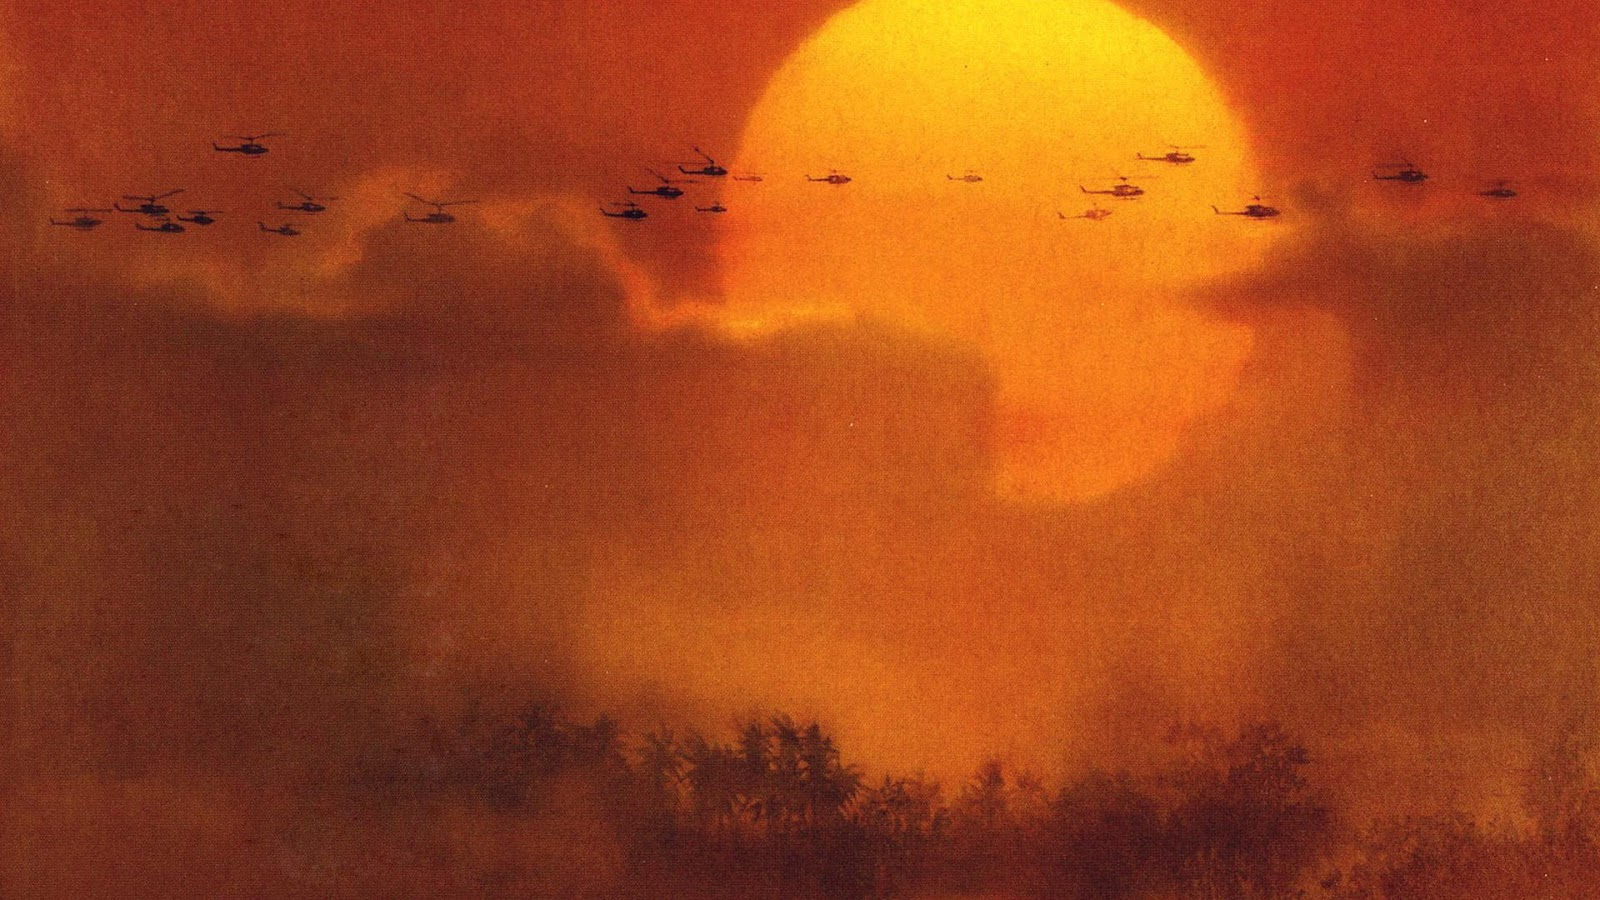
\includegraphics[scale=0.2]{apocalypse+now.jpg}
  \end{center}
}

\frame{
    \tableofcontents 
    \vfill
    \hfill
    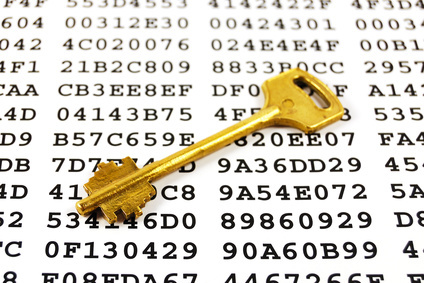
\includegraphics[scale=0.2]{key.jpg}
}


\section{Ausgangslage}
\frame
{
  \frametitle{Das Jahr 2013...}

  \begin{itemize}
    \item Massenhafte Überwachung durch die NSA
    \item einziger (?) Ausweg: Verschlüsselung
    \item Problem: Verschlüsselung ist kompliziert (bestes Beispiel: Greenwald)
    \item weiteres Problem: Verschlüsselung ist nicht immer sicher
  \end{itemize}

  \vfill
  \hfill
  
\includegraphics[scale=0.15]{broken.jpg}

}

\section{Grundlagen}
\subsection{Symmetrische und Asymmetrische Kryptographie}
\frame
{
    \frametitle{Symmetrische und asymmetrische Kryptographie}

    Symmetrische Kryptographie:
    \begin{itemize}
        \item gleicher Schlüssel zum Ver- und Entschlüsseln
        \item schnell
        \item Beispiele: AES, DES, Tripple-DES, Blowfish, RC2, RC4, RC5, RC6
    \end{itemize}

    \vfill

    Asymmetrische Kryptographie:
    \begin{itemize}
        \item beide Parteien müssen keine gemeinsamen Schlüssel kennen
        \item Benutzer erzeugt Schlüsselpaar: geheimer und öffentlicher Schlüssel
        \item langsam
        \item Beispiele: RSA, DSA, Diffie-Hellman
    \end{itemize}
}

\subsection{Asymmetrische Kryptographie}
\frame {
    \frametitle{Asymmetrische Kryptographie}

    \begin{center}
    \only<1> { 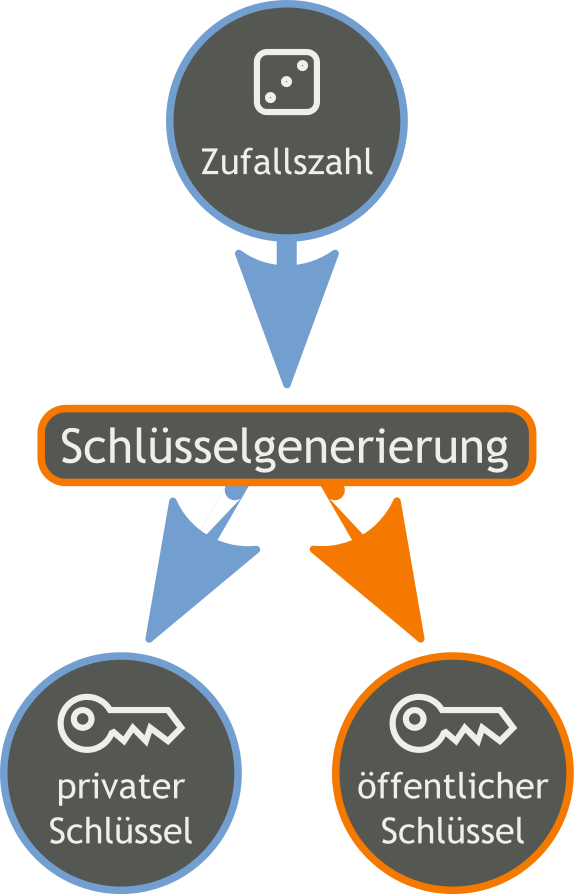
\includegraphics[scale=0.22]{Orange_blue_public_private_keygeneration_de.png} }
    \only<2> {
    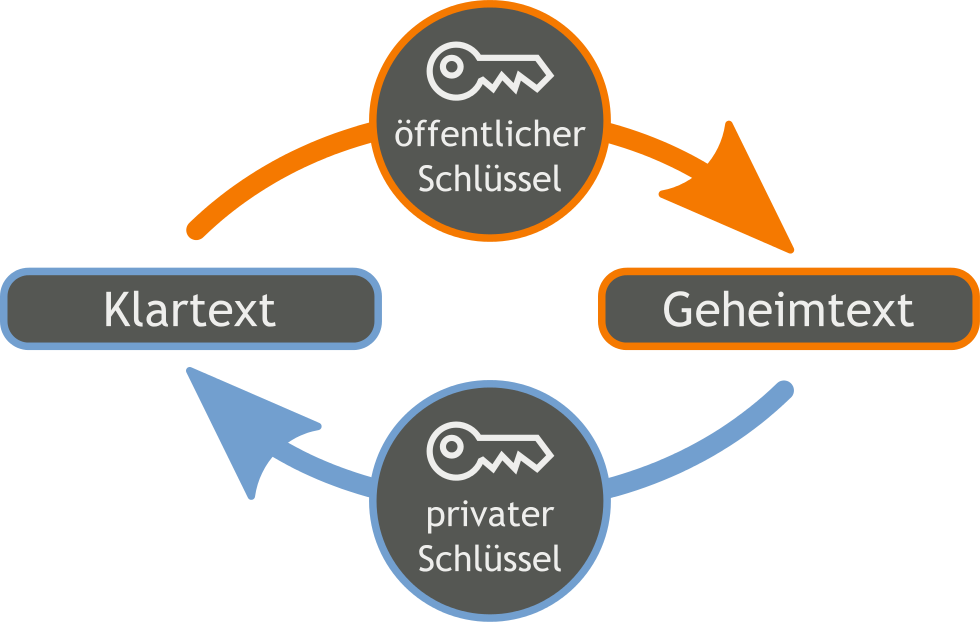
\includegraphics[scale=0.21]{Orange_blue_public_key_cryptography_de.png}
    \hfill
    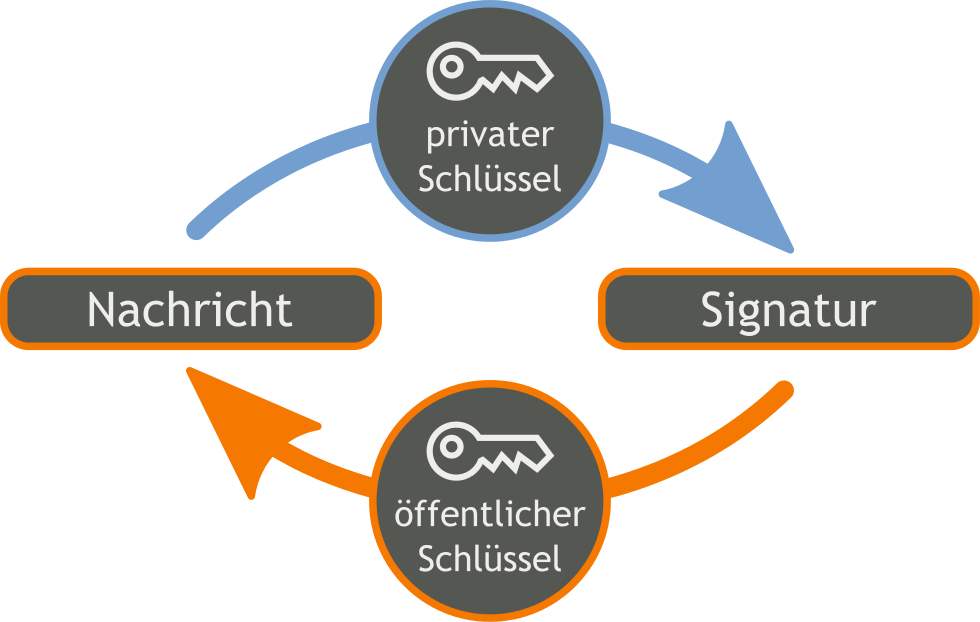
\includegraphics[scale=0.21]{Orange_blue_digital_signature_de.png}
    }
    \end{center}
}

\subsection{Diffie-Hellman}
\frame {
    \frametitle{Beispiel: Diffie-Hellman}

    Funktionsweise:
    \begin{enumerate}
        \item Alice und Bob einigen sich auf eine Primzahl $p$ und eine Primitivwurzel $g$.
        \item Alice erzeugt eine Zufallszahl $a$, Bob erzeugt eine Zufallszahl $b$.
        \item Alice berechnet $A=g^a \mod p$, Bob berechnet $B=g^b \mod p$. Alice und Bob übertragen $A$ und $B$.
        \item Alice berechnet $K=B^a \mod p$, Bob berechnet $K=A^b \mod p$.
    \end{enumerate}

    \hfill

    Beide $K$ gleich:
    \begin{align}
    \nonumber
    K &= B^a \bmod p = (g^b \bmod p )^a \bmod p = g^{ba} \bmod p = g^{ab} \bmod p \\
    \nonumber
    K &= A^b \bmod p = (g^a \bmod p )^b \bmod p = g^{ab} \bmod p
    \end{align}
}

\section{TLS und HTTPS}
\frame
{
    \frametitle{TLS}

    \begin{itemize}
        \item TLS (\textbf{T}ransport \textbf{L}ayer \textbf{S}ecurity, früher SSL): Verschlüsselungsprotokoll zur sicheren Datenübertragung
        \item bekannte Anwendungsfälle: POP3, SMTP, NNTP, SIP, IMAP, XMPP, IRC, LDAP, FTP, OpenVPN
        \item Funktionsweise:
        \begin{enumerate}
            \item Client baut Verbindung zum Server auf
            \item Server authentifiziert sich gegenüber Server mit einem Zertifikat
            \item Server schickt Client mit Zertifikat verschlüsseltes Geheimnis -- oder Diffie-Hellman
            \item aus dem Geheimnis wird ein Schlüssel berechnet
            \item Schlüssel wird für symmetrische Kryptographie benötigt, Absicherung durch MACs
        \end{enumerate}
    \end{itemize}
}

\frame {
    \frametitle{Probleme mit TLS}

    CBC:
    \begin{itemize}
        \item Frühjahr: erfolgreicher Angriff auf CBC in in TLS
        \item Unsicherheit seit 2008 bekannt, Angriffsszenario für unwahrscheinlich eingestuft
        \item Rat: auf RC4-SHA umstellen
    \end{itemize}

    \hfill

    RC4:
    \begin{itemize}
        \item RC4: Stromverschlüsselung
        \item Zufallsstrom von RC4 ist aber nicht immer Zufall
        \item darauf aufbauender Angriff
    \end{itemize}
}

\frame {
    \frametitle{HTTPS heute}

    \begin{itemize}
        \item RC4 und CBC angreifbar
        \item TLS 1.2 wird noch nicht wirklich unterstützt
        \item Server beharren teilweise auf RC4 (trauriges Beispiel: Allianz für Cybersicherheit)
        \item und: CA-System kaputt
    \end{itemize}

    \vfill
    \hfill
    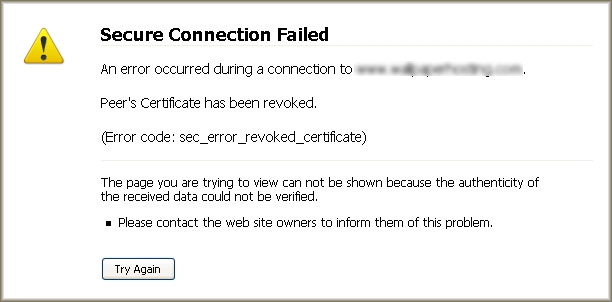
\includegraphics[scale=0.3]{Secure-Connection-Failed.jpg}
}

\section{Mails}

\frame {
    \frametitle{E-Mail}

    \begin{center}
    
\includegraphics[scale=0.3]{email.jpg}
    \end{center}
}
\frame {
    \frametitle{Lavabit}

    \begin{itemize}
        \item kurz nach den ersten Enthüllungen von Snowden schließt Lavabit
        \item Lavabit: E-Mail Provider für sichere Kommunikation, den Snowden nutzte
        \item Behörden wollten Betreiber Levinson zur Herausgabe der Master-SSL-Schlüssel zwingen
        \item damit wäre komplette Kummunikation -- auch bisherige -- entschlüsselbar gewesen
        \item Levabit stellte Dienst ein und erkläre Schlüssel für ungültig
    \end{itemize}
}

\frame {
    \frametitle{Offene Fragen und Fazit}

    Offene Fragen:
    \begin{itemize}
        \item Wie viele solcher Gerichtsbeschlüsse wurden ausgehändigt?
        \item Wie viele Provider schweigen oder müssen schweigen?
        \item Verschlüssellung zwischen E-Mail Providern?
    \end{itemize}

    \hfill

    Fazit:
    \begin{itemize}
        \item Diffie-Hellman anstatt DSA für den Schlüsselaustausch $\Rightarrow$ Perfect Forward Security
        \item E-Mail ist unsicher
        \item DE-Mail ist keine Alternative (Entschlüsselung der Mails auf den Servern der Unternehmen)
    \end{itemize}
}

\section{Backdoors}
\frame {
    \frametitle{Hintertürchen}

    \begin{center}
    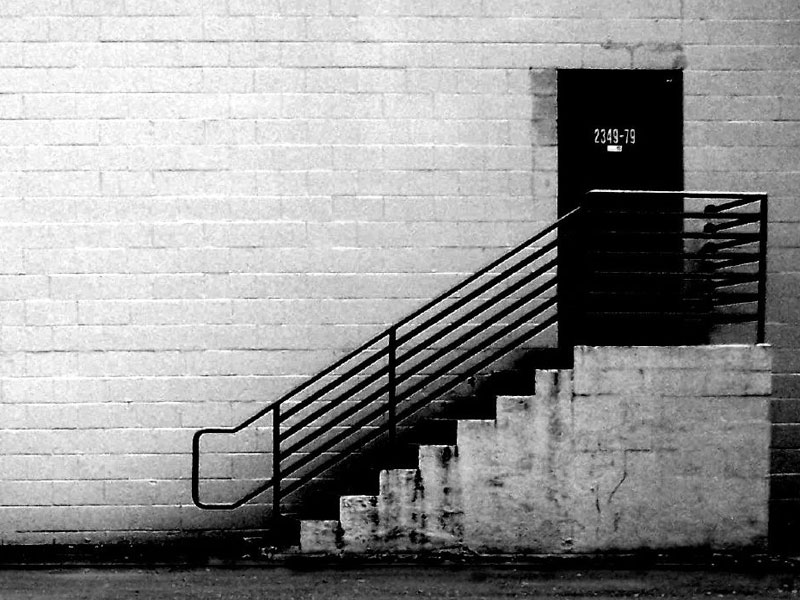
\includegraphics[scale=0.3]{hintertuer.jpg}
    \end{center}
}

\frame {
    \frametitle{Hintertürchen}

    \begin{itemize}
        \item mögiche Hintertür im Zufallszahlengenerator Dual\_EC\_DRBG
        \item NSA soll am Standard nicht nur mitgearbeitet, sondern ihn alleine erstellt haben
        \item Zufallszahlengenerator kommt in kritischen Infrastrukturen weltweit zum Einsatz
        \item NIST und RSA rieten vom Gebrauch von Dual\_EC\_DRBG ab
        \item OpenSSL musste für FIPS-Zertifizierung Dual\_EC\_DRBG implementieren, die Implementation führte aber zum Absturz
        \item NSA und RSA
        \item NIST, SHA3 und Keccak
    \end{itemize}
}

\frame {
    \frametitle{Hintertürchen II}

    \begin{itemize}
        \item QFire:
        \begin{enumerate}
            \item Turmoil: passive Variante, womit NSA alle elektronischen
            Spuren von Telekommunikationsnutzern weltweit sammle $\Rightarrow$
            15-jährige Vorratsdatenspeicherung, Deep-Packet-Inejection
            \item Turbine: Projekt, um Router und Webseiten zu kapern und den Betroffenen Schadcode zu unterjubeln
        \end{enumerate}
        \item GMail: GCHQ schnüffelt für die NSA
        \item Router zumindest von Huawei und Juniper, Server oder PCs und Mobiltelefone werden überwacht
        \item Firmware von Festplatten, Infrarotverbindungen von Servern, Rootkits im BIOS
        \item Auslesen von SMS, Kontakten und Aufnahmen der Kamera von iPhones
        \item Exploits auch für Sun Solaris
    \end{itemize}

    \vfill
    \hfill
    
\includegraphics[scale=0.04]{Key-Features-of-the-New-Solaris-10-10-08.jpg}
}

\frame {
    \frametitle{NSA und Tempest}

    \begin{itemize}
        \item Bauteil Ragemaster wird im Ferrit, einer kleinen Ausbuchtung hinter dem Monitor-Stecker, versteckt
        \item Bauteil erzeugt ein Signal, das unter Verwendung eines externen Radarsystems aufgefangen werden kann
        \item aus den zurückgesendeten Strahlen lass sich der Bildschirminhalt rekonstruieren
        \item ähnliches System für Tastatureingaben
        \item Radardanlagen arbeiten zwischen 1-4 GHz mit Leistung von 1-2kW
        \item Hugo Chávez starb an Krebs
    \end{itemize}
    \vfill
    \hfill
    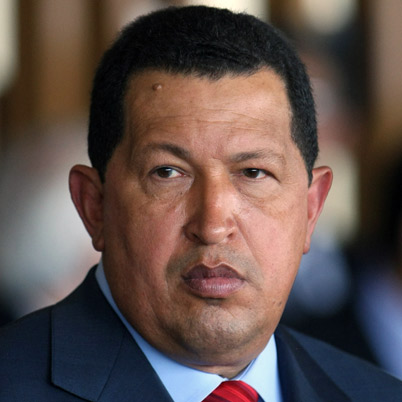
\includegraphics[scale=0.15]{Hugo-Chavez-193225-1-402.jpg}
}

\frame {
    \begin{center}
    
\includegraphics[scale=0.4]{nsa-killed-my-internet.jpg} 
    \end{center}
}

\frame {
    \frametitle{Happy 1984!}

    \begin{center}
    
\includegraphics[scale=0.36]{1308.jpg} 
    \end{center}
}
\end{document}
